% Paquets généraux
\documentclass[a4paper,12pt,titlepage,twoside]{article}
\usepackage[T1]{fontenc}
\usepackage[utf8]{inputenc}
\usepackage[french]{babel}
\usepackage{subcaption}
\addto\captionsfrench{%
  \renewcommand{\tablename}{Tableau}%
}
\usepackage[gen]{eurosym}
%\usepackage[dvips]{graphicx}
\usepackage{minted}
\usepackage{fancyhdr}
\usepackage{pdfpages} 
\usepackage{multido}
\usepackage{hyperref}
\usepackage{textcomp}
\usepackage{schemabloc}
%\usepackage[bitstream-charter]{mathdesign}
\usepackage{array}
\newcolumntype{P}[1]{>{\centering\arraybackslash}p{#1}}
\usepackage[shortlabels]{enumitem}
\usepackage[framemethod=TikZ]{mdframed}

\newcommand{\id}{71}
\newcommand{\nom}{Théorie des mécanismes}
\newcommand{\sequence}{04}
\newcommand{\nomsequence}{Liaisons entre les solides}
\newcommand{\num}{02}
\newcommand{\type}{KH}
\newcommand{\descrip}{Liaisons équivalentes, hyperstatisme, liaisons en série et en parallèle, théorie des graphes}
\newcommand{\competences}{B2-12: Proposer une modélisation des liaisons avec leurs caractéristiques géométriques. \\ &  B2-13: Proposer un modèle cinématique paramétré à partir d'un système réel, d'une maquette numérique ou d'u \\ &  B2-17: Simplifier un modèle de mécanisme. \\ &  B2-18: Modifier un modèle pour le rendre isostatique. \\ &  C1-04: Proposer une démarche permettant d'obtenir une loi entrée-sortie géométrique.  \\ &  C2-05: Caractériser le mouvement d'un repère par rapport à un autre repère. \\ &  C2-06: Déterminer les relations entre les grandeurs géométriques ou cinématiques. }
\newcommand{\nbcomp}{7}
\newcommand{\systemes}{}
\newcommand{\systemesnum}{}
\newcommand{\systemessansaccent}{}
\newcommand{\ilot}{2}
\newcommand{\ilotstr}{02}
\newcommand{\dossierilot}{\detokenize{Ilot_02 }}

%\usepackage{style}
\usepackage{bodegraph}
\usepackage{rpcinematik}
\usepackage[locale = FR]{siunitx}
\usepackage{caption}
\newcommand{\institute}{Lycée Dorian}

\usepackage{listings}
\usepackage{fancyvrb}
\usepackage{color}
\usepackage{xcolor}
\usepackage{colortbl}
\usepackage{helvet}
\usepackage[frenchmath]{newtxsf} % for sans serif symbols
\renewcommand{\familydefault}{\sfdefault}
%\usepackage{amsfonts}
%\usepackage{amsmath}
%\usepackage{lmodern}
\usepackage{mathastext}
%\usepackage{xspace}
\usepackage{varioref}
\usepackage{tabularx}
%\usepackage{floatflt}
\usepackage{graphics}
\usepackage{wrapfig}
\usepackage{textcomp}
\usepackage{tikz,tkz-tab}
\usepackage[european resistor, european voltage, european current]{circuitikz}
\usepackage{wrapfig}
\usepackage{gensymb}
\usepackage[percent]{overpic}
\usetikzlibrary{babel}
\usepackage{ifthen}
\usepackage{cancel}
\usepackage{etoolbox}
\usepackage{multirow}
%\usepackage{boxedminipage}
\definecolor{gris25}{gray}{0.75}
\definecolor{bleu}{RGB}{18,33,98}
\definecolor{bleuf}{RGB}{42,94,171}
\definecolor{bleuc}{RGB}{231,239,247}
\definecolor{bleum}{RGB}{160,195,226}
\definecolor{rougef}{RGB}{185,18,27}
\definecolor{rougec}{RGB}{255,188,204}%255,230,231
\definecolor{vertf}{RGB}{103,126,82}
\definecolor{vertc}{RGB}{220,255,191}
\definecolor{forestgreen}{rgb}{0.13,0.54,0.13}
\definecolor{blcr}{rgb}{0.59,0.69,0.84}
\definecolor{blfr}{rgb}{0.32,0.51,0.75}
\definecolor{orfr}{rgb}{0.90,0.42,0.15}
\definecolor{orcr}{rgb}{0.90,0.65,0.50}
\definecolor{orangef}{rgb}{0.659,0.269,0.072}
\definecolor{orange}{rgb}{0.58,0.35,0.063}
\definecolor{orangec}{rgb}{0.43,0.32,0.25}
\definecolor{rcorrect}{rgb}{0.6,0,0}
\definecolor{sequence}{rgb}{0.75,0.75,0.75}
\definecolor{competences}{rgb}{0.61,0.73,0.35}
\definecolor{rose}{HTML}{ff00ff}
\definecolor{grisf}{HTML}{222222}
\definecolor{grisc}{HTML}{636363}
\definecolor{normal}{HTML}{4087c4}
\definecolor{info}{HTML}{5bc0de}
\definecolor{success}{RGB}{92,184,92}
\definecolor{warning}{RGB}{240,173,78}
\definecolor{danger}{RGB}{217,83,79}
\hypersetup{                    % parametrage des hyperliens
    colorlinks=true,                % colorise les liens
    breaklinks=true,                % permet les retours à la ligne pour les liens trop longs
    urlcolor= blfr,                 % couleur des hyperliens
    linkcolor= orange,                % couleur des liens internes aux documents (index, figures, tableaux, equations,...)
    citecolor= forestgreen                % couleur des liens vers les references bibliographiques
    }

\newcolumntype{M}[1]{>{\centering\arraybackslash}m{#1}}
\definecolor{codegreen}{rgb}{0,0.6,0}
\definecolor{codegray}{rgb}{0.5,0.5,0.5}
\definecolor{codepurple}{rgb}{0.58,0,0.82}
\definecolor{backcolour}{rgb}{0.95,0.95,0.92}

\lstdefinestyle{mystyle}{
    backgroundcolor=\color{backcolour},   
    commentstyle=\color{codegreen},
    keywordstyle=\color{magenta},
    numberstyle=\tiny\color{codegray},
    stringstyle=\color{codepurple},
    basicstyle=\ttfamily\footnotesize,
    breakatwhitespace=false,         
    breaklines=true,                 
    captionpos=b,                    
    keepspaces=true,                 
    numbers=left,                    
    numbersep=5pt,                  
    showspaces=false,                
    showstringspaces=false,
    showtabs=false,                  
    tabsize=2
}

\lstset{style=mystyle}

% Mise en page
\pagestyle{fancy}

\setlength{\hoffset}{-18pt}
\setlength{\oddsidemargin}{0pt} 	% Marge gauche sur pages impaire2s
\setlength{\evensidemargin}{0pt} 	% Marge gauche sur pages paires
\setlength{\marginparwidth}{00pt} 	% Largeur de note dans la marge
\setlength{\headwidth}{481pt} 	 	% Largeur de la zone de tête (17cm)
\setlength{\textwidth}{481pt} 	 	% Largeu\textbf{r de la zone de texte (17cm)
\setlength{\voffset}{-18pt} 		% Bon pour DOS
\setlength{\marginparsep}{7pt}	 	% Séparation de la marge
\setlength{\topmargin}{-30pt} 		% Pas de marge en haut
\setlength{\headheight}{55pt} 		% Haut de page
\setlength{\headsep}{20pt} 		% Entre le haut de page et le texte
\setlength{\footskip}{30pt} 		% Bas de\textbf{ page + séparation
\setlength{\textheight}{700pt} 		% Hauteur de l'icone zone de texte (25cm)
\setlength\fboxrule{1 pt}
\renewcommand{\baselinestretch}{1}
\setcounter{tocdepth}{1}
\newcommand{\cadre}[2]
{\fbox{
  \begin{minipage}{#1\linewidth}
   \begin{center}
    #2\\
   \end{center}
  \end{minipage}
 }
}

\newcommand{\repon}[1]
{
~\ \\
\begin{tabular}{|m{\linewidth}|}
 \hline
\multido{}{#1}{\\ \hline}
\end{tabular}
}


\newcommand{\objectif}[1]{
\mdfsetup{%
frametitle={%
\tikz[baseline=(current bounding box.east),outer sep=0pt]
\node[anchor=east,rectangle,fill=bleum]
{\strut Objectif~};}}
\mdfsetup{innertopmargin=10pt,linecolor=bleum,%
linewidth=2pt,topline=true,%
frametitleaboveskip=\dimexpr-\ht\strutbox\relax
}
\begin{mdframed}[]\relax%
#1
\end{mdframed}}


\newcounter{num_quest} \setcounter{num_quest}{0}
\newcounter{num_rep} \setcounter{num_rep}{0}
\newcounter{num_cor} \setcounter{num_cor}{0}

\newcommand{\feuilleDR}[1]{
	\begin{tikzpicture}
		\draw[gray!30](0,0)grid[step=0.5cm](\linewidth,#1);
	\end{tikzpicture}
}

%\newcommand{\question}[1]{\refstepcounter{num_quest}\par
%~\ \\ \parbox[t][][t]{0.15\linewidth}{\textbf{Question \arabic{num_quest}}}\parbox[t][][t]{0.85\linewidth}{#1\label{q\the\value{num_quest}}}\par
%}

\newcommand{\question}[1]{\refstepcounter{num_quest}\par
~\ \\ \textbf{Question \arabic{num_quest} : }#1\label{q\the\value{num_quest}}\par
}

\newcommand{\posetafigure}[3]{
\begin{figure}[ht!]
 \begin{center}
  \includegraphics[width=#2\linewidth]{img/#1}
 \end{center}
 \caption{\label{#1} #3}
\end{figure}}

\newcommand{\goforum}{
\begin{figure}

\end{figure}
\begin{center}
 
\includegraphics[width=0.7\linewidth]{../../../img/go_forum}
\end{center}
\label{go_forum}
\caption{J'pète les plombs}
\end{figure}}

\newcommand{\reponse}[4][1]
{\noindent
\parbox{\textwidth}{
\rule{\linewidth}{.5pt}\\
\textbf{Question\ifthenelse{#1>1}{s}{} \multido{}{#1}{%
\refstepcounter{num_rep}\ref{q\the\value{num_rep}} }:} ~\ \\
\ifdef{\public}{#3 \ifthenelse{#2>0}{~\ \\ 	\feuilleDR{#2}}}{#4}
}}

\newcommand{\cor}
{\refstepcounter{num_cor}
\noindent
\rule{\linewidth}{.5pt}
\textbf{Question \arabic{num_cor}:} \\
}

\newcommand{\finsujet}
{
    \begin{center}
    \Large{FIN}
    \end{center}

    \cleardoublepage

    \ifdef{\public}{\pagestyle{docreponse}}{\pagestyle{correction}}

    \ifdef{\public}{
        \begin{tikzpicture} 
            \draw (0,0) rectangle (2,2);
            \draw (0,0) -- (2,2);
            \draw (1.5,0.5) node {\large 20};
            \draw (2.5,0) rectangle (16,2);
            \draw (4.5,1.7) node {\large Commentaires:};
        \end{tikzpicture}
    }
    ~\ \\
}


%\newcommand{\repcarre}[2]
%{
%~\ \\
%\begin{tikzpicture}
%\draw [fill=white] (0,0) rectangle +(\linewidth,#1);
%\node[align=left] at (1.1,#2-0.3) {\textbf{Question #1:}};
%\end{tikzpicture}
%}

\newcommand{\titre}[1]
{\begin{center}
\cadre{0.8}{\huge #1} 
\end{center}
}


%Définition des torseurs :
\newcommand{\torseur}[2]{\left\{\mathcal{#1}_{#2} \right\}}
\newcommand{\torseurh}[3]{\left\{\genfrac{}{}{0pt}{0}{#1}{#2}\right\}_{#3}}
\newcommand{\torseurv}[8]{\left\{
\begin{matrix}
#1 & #4 \\ #2 & #5 \\ #3 &#6
\end{matrix}
\right\}_{{#7},{#8}}}

%Définition des torseurs :
%\newcommand{\torseur}[2]{\left \{\mbox{\relsize{2}{$\mathcal {#1}$}\relsize{-2}}\phantom{}_{\mbox{\scriptsize $#2$}} \right \}}
%\newcommand{\torseurh}[3]{\left\{\genfrac{}{}{0pt}{0}{#1}{#2}\right\}_{#3}}
%\newcommand{\torseurv}[8]{
%\left\{\begin{array}{@{}c|c@{}} #1 & #4 \\ #2 & #5 \\ #3 & #6 \end{array} \right\}_{#7,#8}
%}
\newcommand{\derivee}[2]{\left.\dfrac{\d #1}{\d t}\right|_{#2}}
\newcommand{\tripleint}{\int\!\!\!\!\!\int\!\!\!\!\!\int}

% Notation cinématique et statique
\newcommand{\cinematique}[2]{\mbox{#1}/\mbox{#2}}
\newcommand{\statique}[2]{\mbox{#1}\rightarrow\mbox{#2}}
\newcommand{\moment}[3]{\vv {#1}_{\scriptsize{#3}}(#2)}
\newcommand{\resultante}[2]{\vv {#1}_{\scriptsize{#2}}}


%Commande de base
\newcommand{\jo}{\left(j\omega\right)} % j \omega dans l'analyse fréquentielle
\newcommand{\tl}{\xrightarrow{\mathcal{L}}} % transformée de laplace sur fleche
\newcommand{\tli}{\xrightarrow{\mathcal{L}^{-1}}} % transformée inverse de laplace sur fleche
\renewcommand{\d}[1][]{\mathrm{d#1}}
\newcommand{\dd}[1][]{\mathrm{d#1}}
\newcommand{\vect}[2]{{#1}\wedge{#2}}
\newcommand{\base}[3]{(\vec #1,\vec #2,\vec #3)}
\newcommand{\vectbase}[4]{{\vphantom{\left| \begin{matrix}
#1\\#2\\#3 \end{matrix} \right|}}_{#4}{\left| \begin{matrix}
#1\\#2\\#3 \end{matrix} \right.}}
%Pour avoir les paragraphes sous la forme I, II, III
\renewcommand{\thesection}{\Roman{section}}
\setcounter{secnumdepth}{3}
\renewcommand{\Frlabelitemii}{$\bullet$}

% En tête et pied de page
\lhead{\nom}
\rhead{
\includegraphics[width=2cm]{../../../img/logo}}
\lfoot{\auteurun,\ \auteurdeux}
\cfoot{Page \thepage}

\fancypagestyle{docreponse}{%
  \fancyhf{}
  \fancyhead[LO]{NOM Prénom: .............................}
  \rhead{
\includegraphics[width=2cm]{../../../img/logo}\hspace{2pt}}
  \ifdef{\auteurdeux}{\lfoot{\auteurun,\ \auteurdeux}}{\lfoot{\auteurun}}
  \rfoot{\nom}
  \lfoot{Document réponse}
  \cfoot{Page \thepage}
   }

\fancypagestyle{correction}{%
  \fancyhf{}
  \lhead{\colorbox{danger}{\begin{minipage}{0.65\paperwidth} \textcolor{white}{\textbf{Correction}} \end{minipage}} }
  \rhead{
\includegraphics[width=2cm]{../../../img/logo}}
  \lfoot{Renaud Costadoat, Françoise Puig}
  \rfoot{\colorbox{danger}{\begin{minipage}{0.4\paperwidth} \begin{flushright}\textcolor{white}{\textbf{Correction}}\end{flushright} \end{minipage}} }}

\fancypagestyle{correctioninfo}{%
  \fancyhf{}
  \lhead{\colorbox{danger}{\begin{minipage}{0.65\paperwidth} \textcolor{white}{\textbf{Correction}} \end{minipage}} }
  \rhead{
\includegraphics[width=2cm]{../../../img/logo}}
  \lfoot{Renaud Costadoat, Juliette Genzmer}
  \rfoot{\colorbox{danger}{\begin{minipage}{0.6\paperwidth} \begin{flushright}\textcolor{white}{\textbf{Correction}}\end{flushright} \end{minipage}} }}

\renewcommand{\footrulewidth}{0.4pt}

\usepackage{eso-pic}
\newcommand{\BackgroundPic}{%
\put(0,0){%
\parbox[b][\paperheight]{\paperwidth}{%
\vfill
\begin{center}
\hspace{0.5cm}\vspace{0.5cm}

\includegraphics[width=\paperwidth,height=\paperheight,%
keepaspectratio]{../../../img/fond3}%
\end{center}
\vfill
}}}

\newcommand{\BackgroundPicdeux}{%
\put(25,-30){%
\parbox[b][\paperheight]{\paperwidth}{%
\vfill
\begin{center}
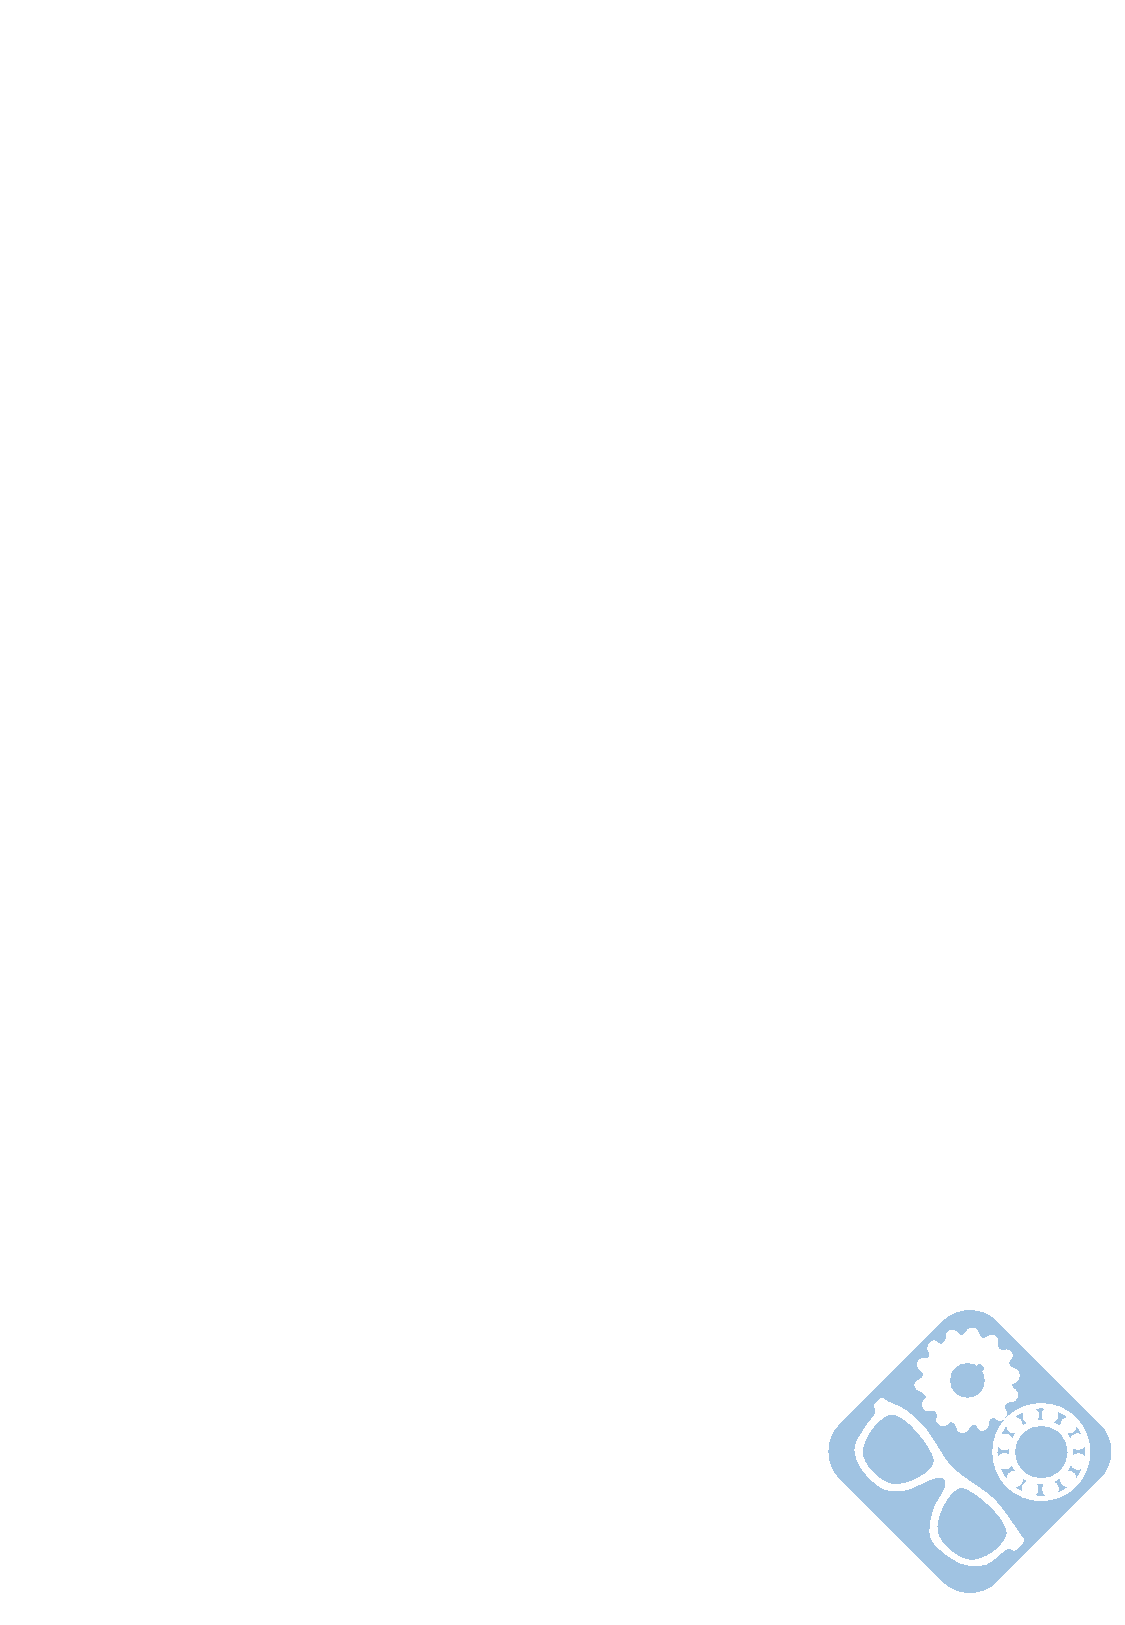
\includegraphics[width=\paperwidth,height=\paperheight,%
keepaspectratio]{../../../img/fond4}%
\end{center}
\vfill
}}}

\begin{document}

\pagestyle{empty}

\AddToShipoutPicture*{\BackgroundPic}


\includegraphics[width=2cm]{../../../img/logo}

\Huge{DS \numero - \sujet}

\vspace{1cm}

\ifdef{\prive}{\begin{center}\colorbox{danger}{\Huge{Avec Correction}}\end{center}}{}

\begin{center}
\centering\huge{PTSI}
\end{center}

\vspace{2cm}


\begin{center}
\centering\Large{\jour}
\end{center}

\vspace{2cm}

\normalsize

\tableofcontents

\newpage

\AddToShipoutPicture{\BackgroundPicdeux}

\pagestyle{fancy}

\begin{center}
\Huge \sujet
\end{center}


\normalsize


\section{Présentation}

Chaque année, le salon CES de Las Vegas, propose de nouveaux robots et appareils
connectés. Les robots lave-vitres y sont apparus en 2012. Ils sont capables de laver des surfaces verticales, horizontales ou obliques, de grandes dimensions aussi bien à l’intérieur qu’à l’extérieur de la maison.

Les robots lave-vitres actuels répondent au même besoin, avec cependant des
performances pouvant être très différentes suivant les solutions technologiques retenues.

Une société d’électroménager a pris en compte les remarques d’un groupe de
consommateurs (tableau \ref{tab01}) possédant déjà des robots lave-vitres (de structure monobloc ou en deux parties) afin de définir les exigences de conception d’un nouveau produit.

\begin{figure}[ht!]
\begin{center}
 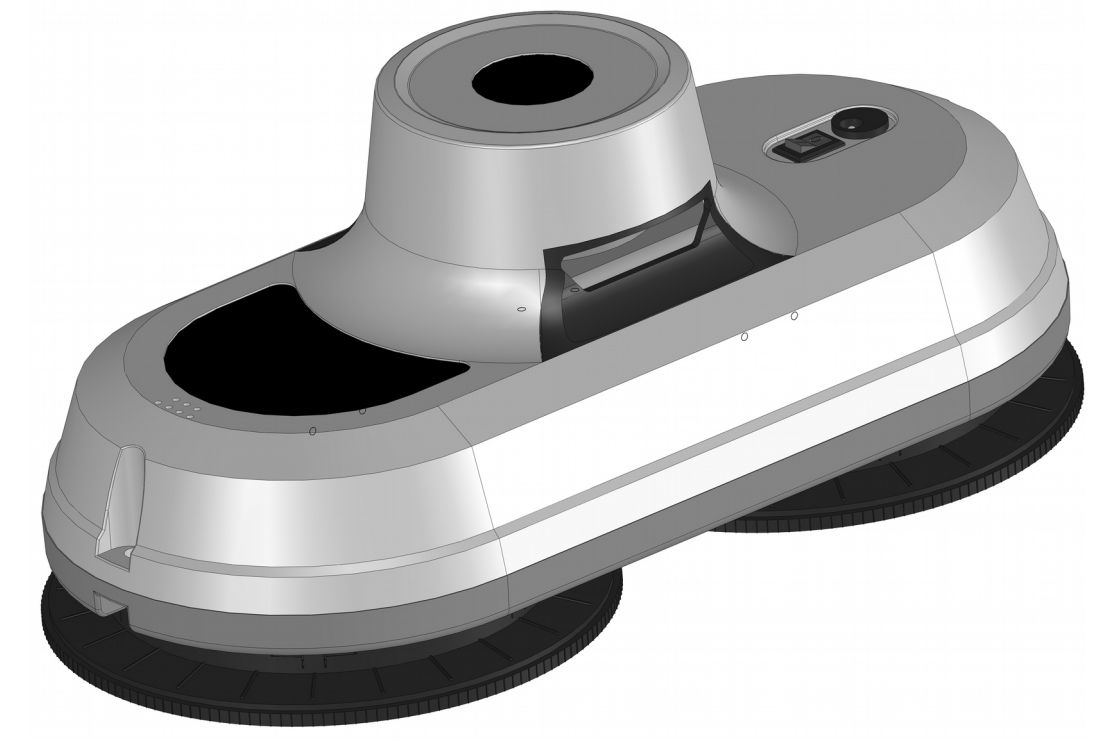
\includegraphics[width=0.4\linewidth]{img/fig01}
\end{center}
\caption{\label{fig01} Robot nettoyeur multi-surfaces}
\end{figure}

\begin{table}[ht!]
\begin{tabularx}{\linewidth}{|X|X|}
\hline
\rowcolor{gray}
\begin{center}
Remarques sur les robots de type monobloc
\end{center}
 & \begin{center}
Remarques sur les robots en deux parties (placées de chaque coté du vitrage)
\end{center}
\\
\hline
Ventouse de la ligne de vie pas assez puissante pour retenir le robot lors d'une chute.
& Difficulté pour positionner les deux parties du robot de chaque coté de la paroi vitrée (cas de vitres d'immeuble). \\
\hline
Dimensions un peu grandes pour les petites surfaces : lucarnes, vasistas, etc.
& Pas de ligne de vie (cordage). Dangereux, car le robot n'est pas retenu lors de pertes
d'adhérence.\\
\hline
Réservoir de produit lavant suffisant pour les plus grandes parois vitrées.
& Toute la surface de la paroi vitrée n'est pas balayée lors d'un décalage accidentel des deux parties du robot.\\
\hline
Traces sur les vitrages dues aux chenilles permettant le déplacement.
& Chute du robot si l'aimantation entre les deux parties du robot est mal réglée.\\
\hline
Surface seulement balayée à 80\% du fait de sa forme. & Pas de traces sur la paroi vitrée lors du déplacement du robot. \\
\hline
Balayage de tout type de surface (vitrée ou non).& \\
\hline
\end{tabularx}
\caption{\label{tab01} Remarques d'un groupe de consommateurs}
\end{table}

\question{En prenant appui sur les remarques négatives communes aux deux structures de robot lave-vitres actuels, citer au moins deux besoins fonctionnels auxquels devra répondre le nouveau robot lave-vitres.}

~\

Après avoir étudié les remarques du groupe de consommateurs, la société a décidé de
fabriquer un prototype dont on peut voir une modélisation sur le document technique DT1.

Il est constitué de deux patins qui, lorsqu'ils sont mis en mouvement comme présenté sur
les schémas du document technique DT2, permettent à la fois le balayage de la
paroi vitrée et le déplacement du robot.

Une turbine assure une dépression dans les patins afin de permettre au robot de se
maintenir sur la paroi vitrée. La distribution de l'énergie au moteur de la turbine se fait grâce à un transistor.

L'apport d'énergie électrique est assuré par un bloc d'alimentation 230 VCA/24 VCC
extérieur au robot. Le bloc alimentation et le robot sont connectés en permanence grâce à un câble électrique. Dans le cas d'une coupure d'énergie électrique, une batterie
d'accumulateurs 14,8 VCC permet d'assurer le maintien du robot sur la paroi vitrée
pendant une vingtaine de minutes.

Après avoir placé des bonnets en microfibres sur les patins, l'utilisateur n'a plus qu'à
poser le robot sur la paroi vitrée tout en appuyant sur le bouton marche-arrêt pour mettre en fonctionnement la turbine. Une télécommande permet ensuite d'envoyer des ordres de déplacement au robot.

~\

L'objectif du sujet est de valider plus précisément les solutions qui permettent :
\begin{itemize}
 \item le déplacement du robot pour assurer le balayage de la totalité de la surface de la paroi vitrée ;
 \item la sécurité du robot.
\end{itemize}

\section{Déplacement du robot sur la paroi vitrée}

\paragraph{Objectif de cette partie :} valider le modèle multiphysique pour que le robot se déplace sur toute la surface vitrée.

\paragraph{Analyse structurelle du robot} ~\ \\

\question{À partir des informations données dans la présentation du système et du document technique DT1, compléter le diagramme de la structure fonctionnelle du robot en plaçant les composants manquants sur le document réponse. Indiquer les grandeurs d'effort et de flux manquantes et préciser la valeur numérique des grandeurs d'effort entrantes et sortantes du bloc \og alimenter \fg\ dans le cas d'un fonctionnement normal et dans le cas d'une coupure d'énergie électrique.}

~\

La fonction convertir est effectuée par deux moteurs à patin. Ce sont des moteurs à courant continu.

On donne les variables suivantes qui caractérisent le comportement du moteur :
\begin{itemize}
 \item $u_m(t)$ : la tension aux bornes du moteur,
 \item $i_m(t)$ : le courant qui traverse le moteur,,
 \item $e(t)$ : la force contre-électromotrice du moteur,
 \item $c_m(t)$ : le couple moteur,
 \item $\omega_m(t)$ : la vitesse de rotation du moteur.
\end{itemize}

\newpage

On donne les constantes suivantes caractéristiques du moteur étudié. Les valeurs numériques sont exprimées en unités SI mais celles-ci ont été effacées pour la question \ref{q3} :
\begin{itemize}
 \item $R=2$ : résistance de l'induit,
 \item $L=6\cdot 10^{-4}$ : inductance de l'induit,
 \item $K_e=44\cdot 10^{-3}$ : constante de vitesse du moteur,
 \item $K_c=44\cdot 10^{-3}$ : constante de couple du moteur,
 \item $J=3\cdot 10^{-4}$ : inertie globale ramenée à l'arbre moteur.
 \item $f=?$ : coefficient de frottements visqueux.
\end{itemize}


\question{Compléter le tableau en indiquant les unités de toutes ces variables et de toutes ces constantes.}

\question{Écrire les quatre équations du moteur qui relient TOUTES ces variables et constantes.}

\question{Passer ces équations dans le domaine de Laplace (les conditions initiales sont nulles pour cette étude). On appellera $U_m(p)$, $I(p)$, $E(p)$, $\Omega_m(p)$ et $C_m(p)$ les transformées de $u_m(t)$, $i(t)$, $e(t)$, $\omega_m(t)$ et $c_m(t)$.}

\question{Déterminer la fonction de transfert $H(p)=\dfrac{\Omega_m(p)}{U_m(p)}$ sous sa forme canonique.}

\question{Donner sa classe, son ordre et les expressions littérales de ses paramètres caractéristiques $K$, $\xi$ et $\omega_0$.}

~\

On donne le relevé expérimental suivant, effectué après avoir alimenté le moteur avec une tension de $u_m(t)=12V$.

\begin{figure}[ht!]
\begin{center}
 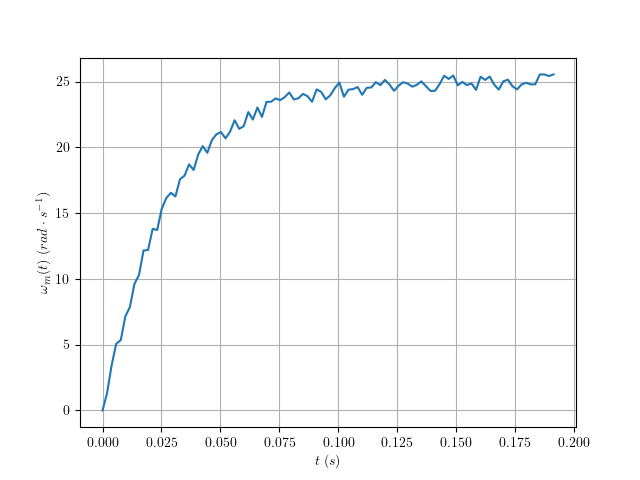
\includegraphics[width=0.6\linewidth]{img/fig02}
\end{center}
\caption{\label{fig02} Tracé de la réponse temporelle du moteur}
\end{figure}

\question{A partir de la réponse temporelle de la figure \ref{fig02} et des résultats de la question \ref{q7}, déterminer le coefficient $f$.}

\question{Faire l'application numérique pour toutes les grandeurs de la question \ref{q7}. Commenter ces résultats à la vue des tracés des figure \ref{fig02} et \ref{fig03}.}

\newpage

\begin{figure}[!ht]
\begin{center}
 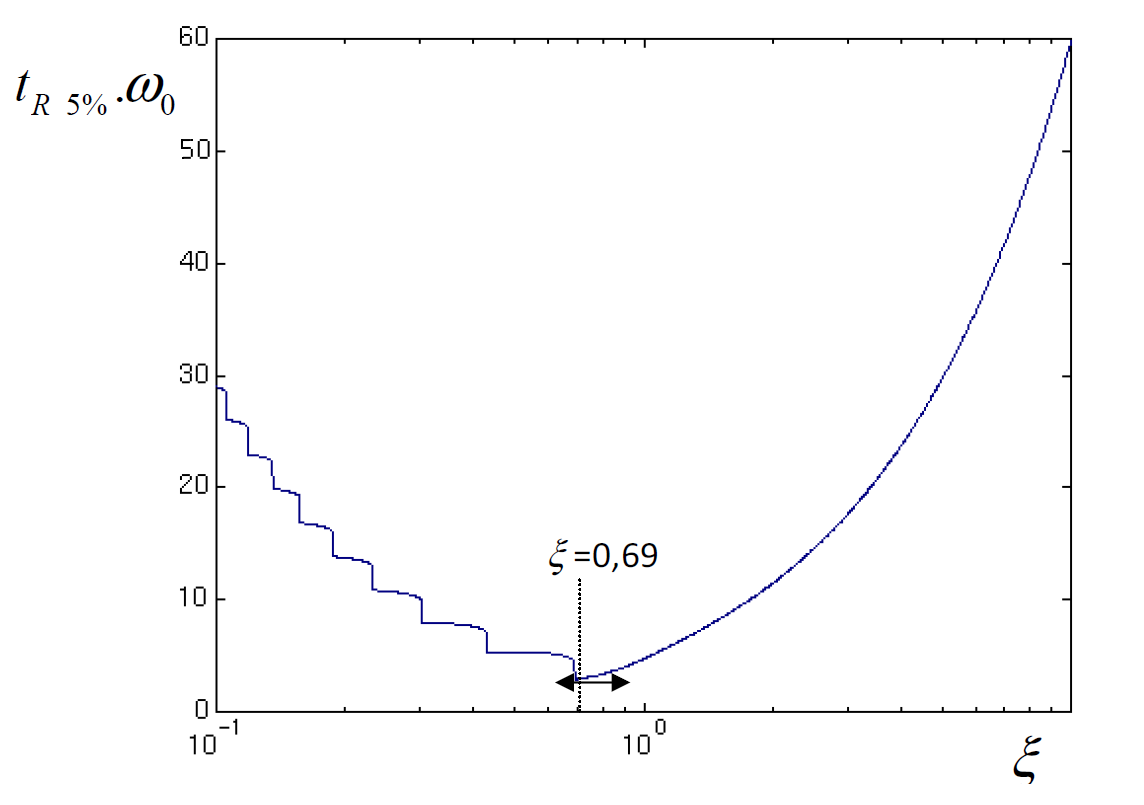
\includegraphics[width=0.6\linewidth]{img/fig03}
\end{center}
\caption{\label{fig03} Tracé du temps de réponse en fonction de $\xi$.}
\end{figure}

Des calculs issus des résultats de la question \ref{q7} montrent que : ~\

\begin{center}
$\dfrac{d\xi}{dJ}=140\cdot \dfrac{1}{\sqrt{J}}-\dfrac{10^{-3}}{2\cdot J^{\frac{3}{2}}}$
\end{center}

\question{Justifier que $\xi$ est minimum pour $J\approx 3\cdot 10^{-6}kg\cdot m^2$.}

\question{Montrer que la valeur de $\xi$ correspondante est 1.}

\question{Déterminer la valeur de $J$ pour que le système soit le plus rapide.}

\subsection{Pilotage du moteur de la turbine}

La mise en mouvement de la turbine par un échelon génère une accélération trop importante qui peut mener au décrochage du robot. On décide pour cela de la piloter en suivant un profil de tension en trapèze.

Le moteur peut être modélisé par la fonction de transfert suivante:
\begin{center}
$G(p)=\dfrac{\Omega_m(p)}{U_m(p)}=\dfrac{2}{1+\dfrac{2}{350}\cdot p+\dfrac{p^2}{350^2}}$
\end{center}

Pour modéliser la phase d'accélération, le profile de u(t) sera celui d'une rampe, ainsi, $U_m(p)=\dfrac{1}{p^2}$.

\question{Montrer à partir d'une décomposition en éléments simples, que la vitesse de rotation du moteur peut s'écrire dans le domaine de Laplace:

$\Omega_m(p)=u\cdot\dfrac{p}{\left(350+p\right)^2}+v\cdot\dfrac{1}{\left(350+p\right)^2}+w\cdot\dfrac{1}{p}+z\cdot\dfrac{1}{p^2}$. Déterminer alors les valeurs des coefficients $u$, $v$, $w$ et $z$.}

On sait que : $L[t\cdot e^{-at}]=\dfrac{1}{(p+a)^2}$

\question{Montrer que $L[e^{-at}\cdot (1-t\cdot a)]=\dfrac{p}{(p+a)^2}$.}

\question{En déduire l'expression temporelle de $\omega_m(t)$ en fonction de $u$, $v$, $w$ et $z$.}

Le document réponse montre la réponse temporelle de $\omega_m(t)$. Deux autres ont été définies comme suit:
\begin{itemize}
 \item pour $f(t)$, 3 valeurs parmi $u$, $v$, $w$ et $z$ ont été mises à 0,
 \item pour $g(t)$, 2 valeurs parmi $u$, $v$, $w$ et $z$ ont été mises à 0.
\end{itemize}

\question{Préciser sur la légende de la courbe les équations des droites tracées.}

\question{En déduire les valeurs des coefficients $w$ et $z$.}

On constate sur le tracé que passées 0.02s, $g(t)$ se confond avec $\omega_m(t)$.

\question{Déterminer le retard de traînage $\delta t$ tel que $f(t)=g(t+\delta t)$.}

\section{Représentation en vue plane}

\question{Compléter la projection en vue plane du document réponse.}

\begin{center}
 \Large{FIN}
\end{center}
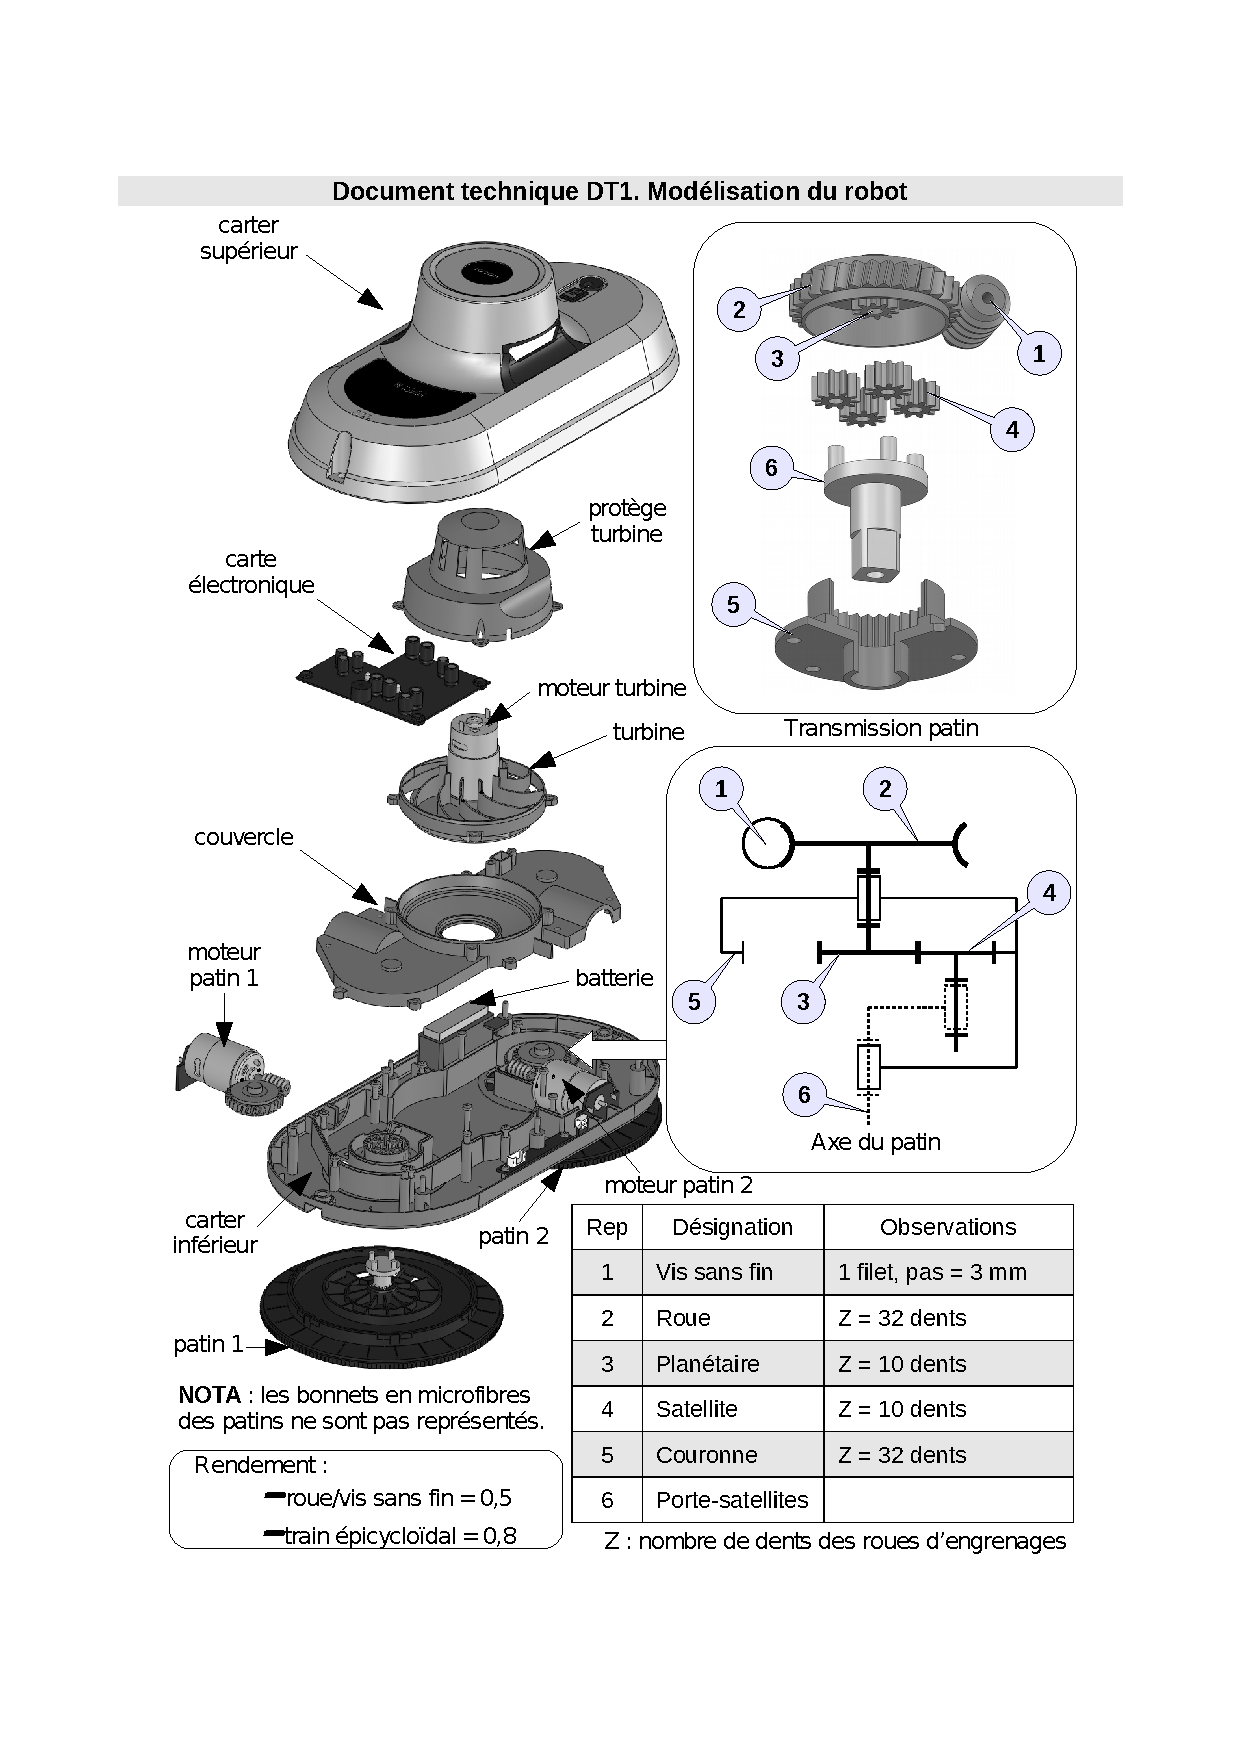
\includepdf[offset=5mm -5mm 0mm 0mm]{img/DT1.pdf}

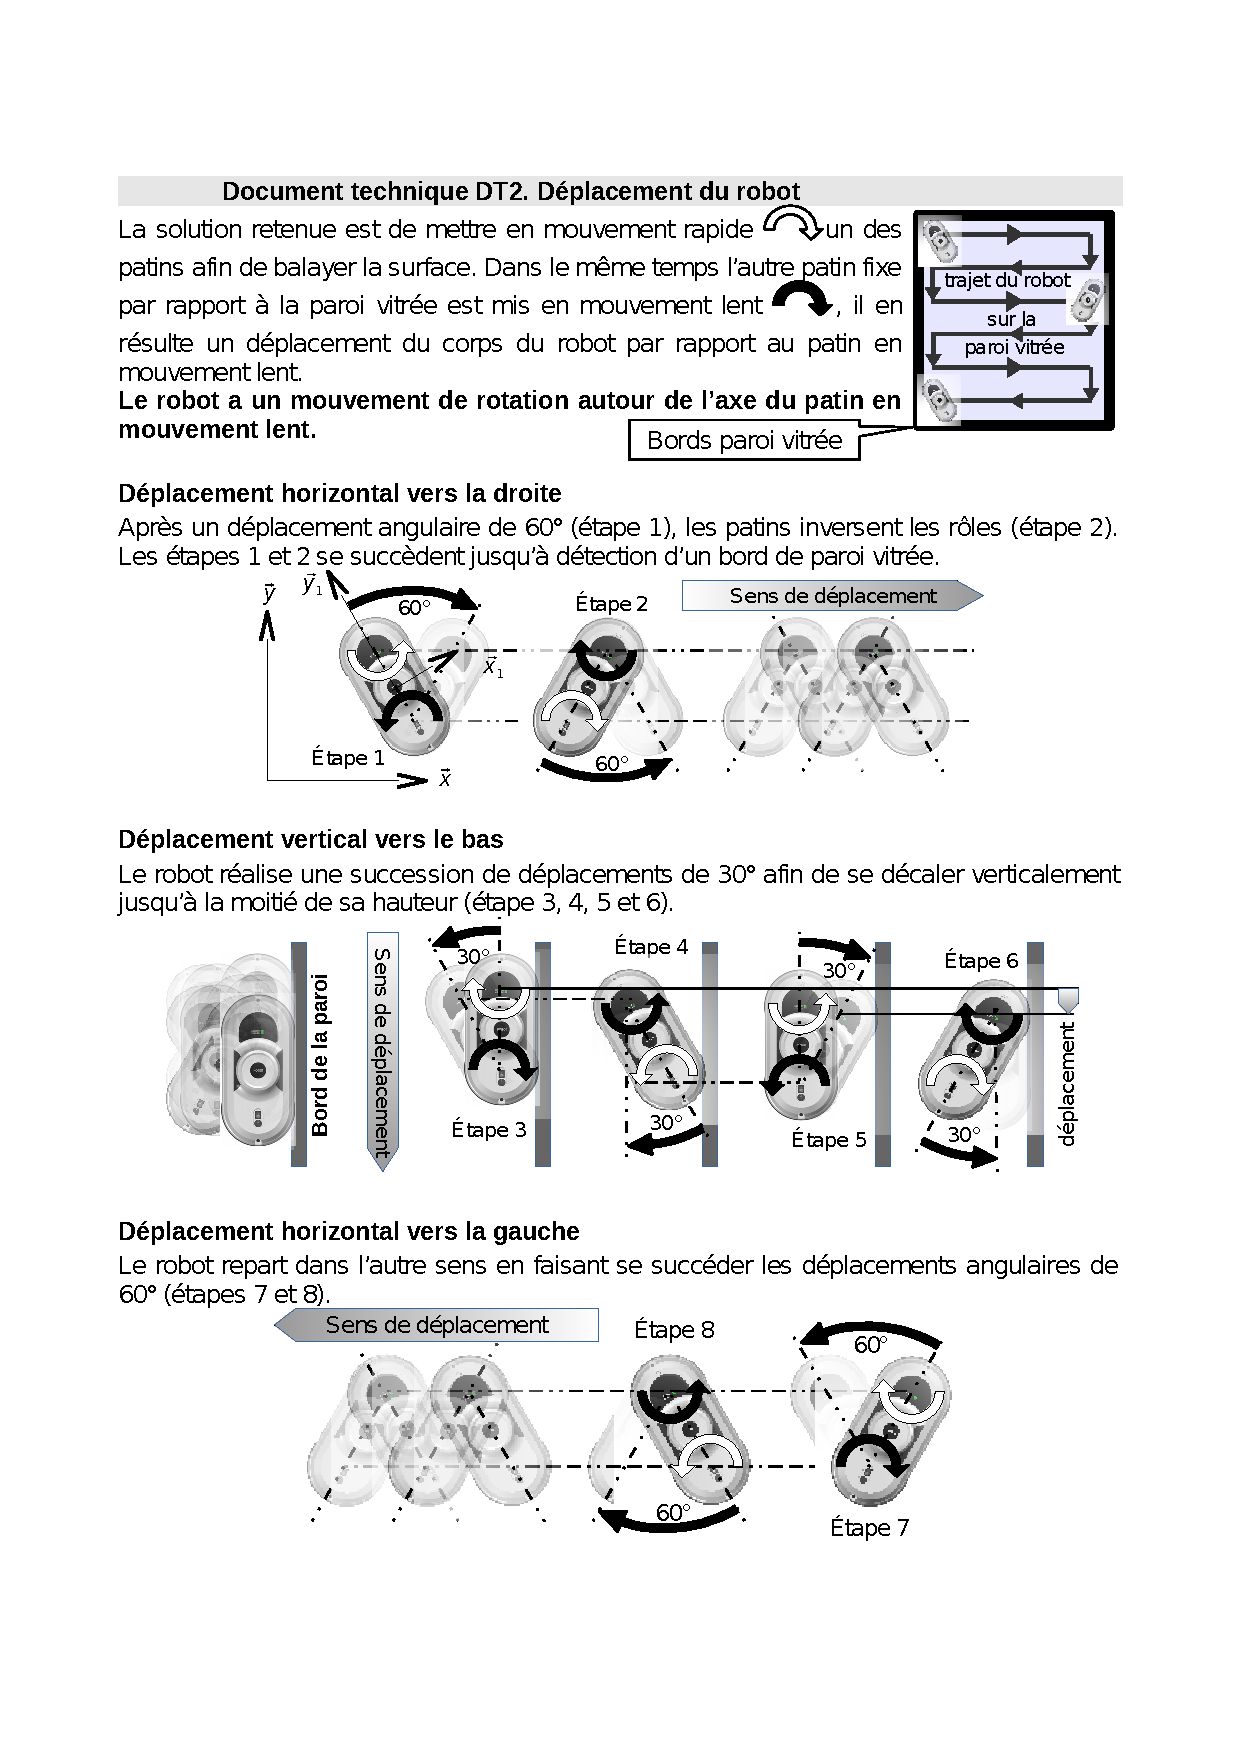
\includepdf[offset=-8mm -10mm 0mm 0mm]{img/DT2.pdf}

\cleardoublepage

\ifdef{\public}{\pagestyle{docreponse}}{\pagestyle{correction}}

\reponse{4}{}{Travailler en toute sécurité. Balayer la totalité de la paroi vitrée.}

\reponse{2}{\begin{figure}[ht!]
\begin{center}
 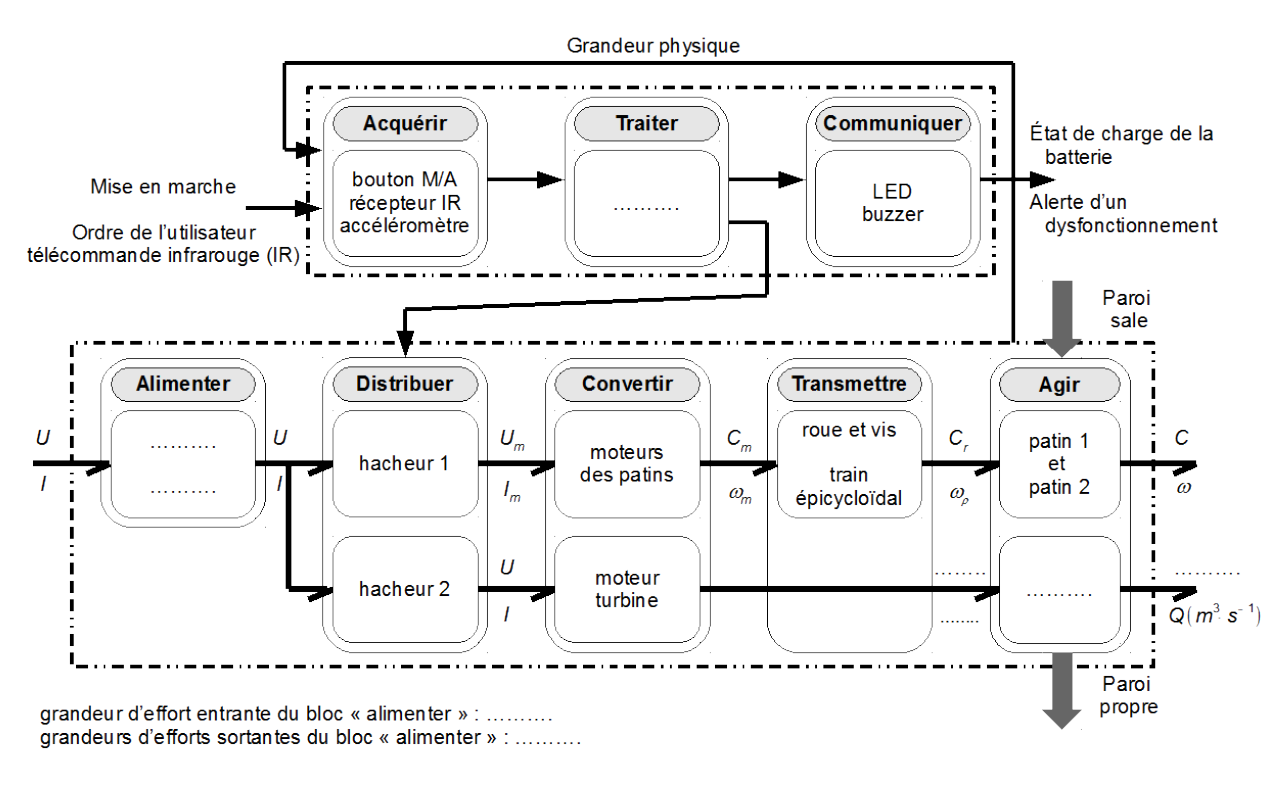
\includegraphics[width=\linewidth]{img/DR01}
\end{center}
\label{dr02}
\caption{Chaînes d'énergie et d'information}
\end{figure}}{\begin{figure}[ht!]
\begin{center}
 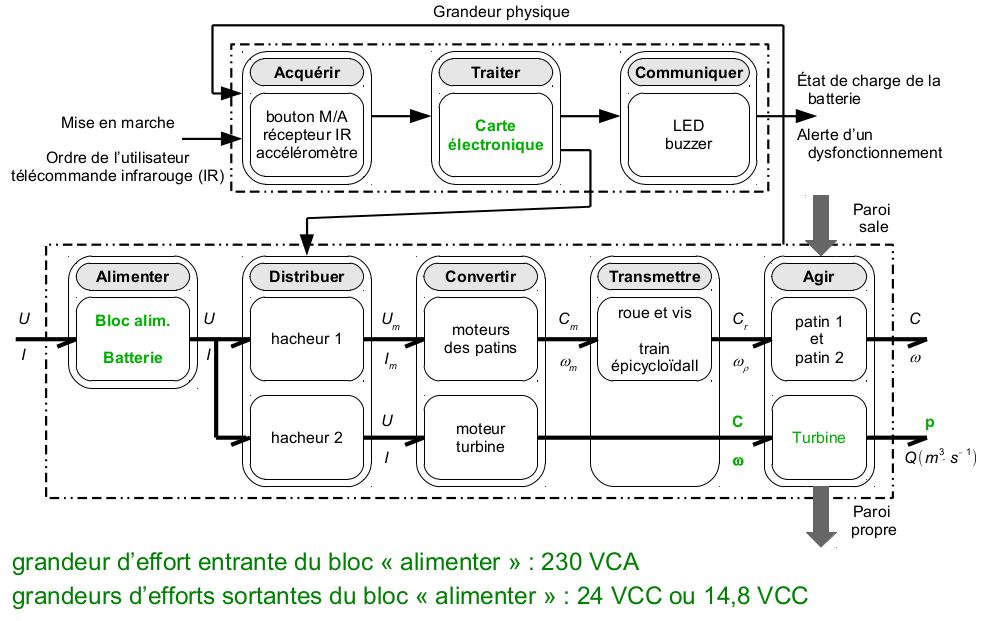
\includegraphics[width=\linewidth]{img/DR01_cor}
\end{center}
\label{dr02}
\caption{Chaînes d'énergie et d'information}
\end{figure}}

\ifdef{\public}{\newpage}

\reponse{0}{
\begin{center}
\begin{tabularx}{.9\linewidth}{|c|X|}
\hline
Grandeur & Unité \\
\hline
$u_m(t)$ & Volt ($V$)\\
\hline
$i_m(t)$ & \\
\hline
$e(t)$ & \\
\hline
$c_m(t)$ & \\
\hline
$\omega_m(t)$ & \\
\hline
$R$ & \\
\hline
$L$ & \\
\hline
$K_e$ & \\
\hline
$K_c$ & \\
\hline
$J$ & \\
\hline
$f$ & \\
\hline
\end{tabularx}
\end{center}}
{\begin{center}
\begin{tabularx}{.7\linewidth}{|c|X|}
\hline
Grandeur & Unité (Symbole)\\
\hline
$u_m(t)$ & Volt ($V$)\\
\hline
$i_m(t)$ & Ampère ($A$)\\
\hline
$e(t)$ & Volt ($V$)\\
\hline
$c_m(t)$ & Newton mètre ($N\cdot m$)\\
\hline
$\omega_m(t)$ & radian par seconde ($rad\cdot s^{-1}$)\\
\hline
$R$ & Ohm ($\omega$)\\
\hline
$L$ & Henri ($H$)\\
\hline
$K_e$ & Volt par radian seconde ($V\cdot rad^{-1} s$) \\
\hline
$K_c$ & Newton mètre par ampère ($N\cdot m \cdot A^{-1}$) \\
\hline
$J$ & Kilogramme mètre carré ($kg\cdot m^2$)\\
\hline
$f$ & Newton mètre par radian seconde ($N\cdot m\cdot rad^{-1} s$).\\
\hline
\end{tabularx}
\end{center}}

\reponse{6}{}{
\begin{eqnarray}
u_m(t)=R\cdot i(t)+L\cdot \dfrac{di(t)}{dt}+e(t) \\
e(t)=K_e\cdot \omega_m(t) \\
c_m(t)=K_c\cdot i(t) \\
J\cdot \dfrac{d\omega_m(t)}{dt}=c_m(t)-f\cdot \omega_m(t)
\end{eqnarray}}

\reponse{6}{}{
\begin{eqnarray}
U_m(p)=R\cdot I(p)+L\cdot p\cdot I(p)+E(p) \\
E(p)=K_e\cdot \Omega_m(p) \\
C_m(p)=K_c\cdot I(p) \\
J\cdot p\cdot \Omega_m(p)=C_m(p)-f\cdot \Omega_m(p)
\end{eqnarray}}

\ifdef{\public}{\newpage}

\reponse{7}{}{
$U_m(p)=(R+L\cdot p)\cdot I(p)+K_e\cdot \Omega_m(p)$ et $(J\cdot p+f)\cdot \Omega_m(p)=C_m(p)=K_c\cdot I(p)$

Donc, $U_m(p)=(R+L\cdot p)\cdot \dfrac{(J\cdot p+f)\cdot \Omega_m(p)}{K_c}+K_e\cdot \Omega_m(p)$

$U_m(p)=\left((R+L\cdot p)\cdot \dfrac{(J\cdot p+f)}{K_c}+K_e\right)\cdot \Omega_m(p)$

$U_m(p)=\dfrac{(R+L\cdot p)\cdot (J\cdot p+f)+K_e\cdot K_c}{K_c}\cdot \Omega_m(p)$

$\dfrac{\Omega_m(p)}{U_m(p)}=\dfrac{K_c}{(R+L\cdot p)\cdot (J\cdot p+f)+K_e\cdot K_c}$

$\dfrac{\Omega_m(p)}{U_m(p)}=\dfrac{K_c}{R\cdot J\cdot p+R\cdot f+L\cdot J\cdot p^2+L\cdot f\cdot p+K_e\cdot K_c}$

$\dfrac{\Omega_m(p)}{U_m(p)}=\dfrac{\dfrac{K_c}{R\cdot f+K_e\cdot K_c}}{1+\dfrac{R\cdot J+L\cdot f}{R\cdot f+K_e\cdot K_c}\cdot p+\dfrac{L\cdot J}{R\cdot f+K_e\cdot K_c}\cdot p^2}$
}

\reponse{6}{}{
\begin{itemize}
 \item Classe 0,
 \item Ordre 2,
 \item $K=\dfrac{K_c}{R\cdot f+K_e\cdot K_c}$,
 \item $\omega_0=\sqrt{\dfrac{R\cdot f+K_e\cdot K_c}{L\cdot J}}$,
 \item $\xi=\dfrac{\omega_0}{2}\cdot \dfrac{R\cdot J+L\cdot f}{R\cdot f+K_e\cdot K_c}=\dfrac{1}{2}\cdot \sqrt{\dfrac{R\cdot f+K_e\cdot K_c}{L\cdot J}}\cdot \dfrac{R\cdot J+L\cdot f}{R\cdot f+K_e\cdot K_c}=\dfrac{R\cdot J+L\cdot f}{2\sqrt{L\cdot J\cdot (R\cdot f+K_e\cdot K_c)}}$
\end{itemize}
}

\reponse{6}{}{Sur la figure, on note la valeur de l'asymptote, $K\cdot 12=25$, donc $K=2.5$.

$K=\dfrac{K_c}{R\cdot f+K_e\cdot K_c}$

$\dfrac{44\cdot 10^{-3}}{2\cdot f+44\cdot 10^{-3}\cdot 44\cdot 10^{-3}}=2$

$44\cdot 10^{-3}=2\cdot (2\cdot f+44\cdot 10^{-3}\cdot 44\cdot 10^{-3})$

$44\cdot 10^{-3}-2\cdot 44\cdot 10^{-3}\cdot 44\cdot 10^{-3}=4\cdot f$

$f=\dfrac{44\cdot 10^{-3}\cdot(1-2\cdot 44\cdot 10^{-3})}{4}$

$f=11\cdot 10^{-3}\cdot(1-0.088)=10^{-3}\cdot(11-1)=10^{-2}N\cdot rad^{-1}\cdot s$
}

\reponse{6}{}{
$\omega_0=\sqrt{\dfrac{2\cdot 10^{-2}+44\cdot 10^{-3}\cdot 44\cdot 10^{-3}}{6\cdot 10^{-4}\cdot 3\cdot 10^{-4}}}=\sqrt{\dfrac{2\cdot 10^{-2}+2000\cdot 10^{-6}}{18\cdot 10^{-8}}}=\sqrt{\dfrac{22\cdot 10^{-3}}{18\cdot 10^{-8}}}=\sqrt{10^{5}}=\sqrt{10}\cdot 10^{5}\approx 300rad\cdot s^{-1}.$ (350 avec moins d'approximations).

$\xi=\dfrac{2\cdot 3\cdot 10^{-4}+6\cdot 10^{-4}\cdot 10^{-2}}{2\sqrt{6\cdot 10^{-4}\cdot 3\cdot 10^{-4}\cdot (2\cdot 10^{-2}+44\cdot 10^{-3}\cdot 44\cdot 10^{-3})}}$
 
 $\xi=\dfrac{6\cdot 10^{-4}}{2\sqrt{18\cdot 10^{-8}\cdot 2\cdot 10^{-2}}}=\dfrac{6\cdot 10^{-4}}{2\sqrt{36\cdot 10^{-10}}}=\dfrac{6\cdot 10^{-4}}{12\cdot 10^{-5}}=\dfrac{10}{2}=5$
 
~\
 
C'est cohérent avec le tracé car $\xi=5$ justifie le fait que l'on ne voit plus la tangente à l'origine, le tracé ressemble à un premier ordre.

Sur l'autre figure, on voit que pour $\xi=5$, $t_{R5\%}\cdot \omega_0=30$, donc $t_{R5\%}=0.1s$ et c'est aussi compatible avec la réponse temporelle si on l'identifie à un premier ordre.
}

\reponse{5}{}{
$0=140\cdot \dfrac{1}{\sqrt{J}}-\dfrac{10^{-3}}{2\cdot J^{3/2}}$

$0=140-\dfrac{10^{-3}}{2\cdot J}$

$280\cdot J=10^{-3}$

$J=\dfrac{10^{-3}}{3\cdot 10^{2}}=3\cdot 10^{-6}$
}

\reponse{5}{}{
$\xi=\dfrac{2\cdot 3\cdot 10^{-6}+6\cdot 10^{-4}\cdot 10^{-2}}{2\sqrt{6\cdot 10^{-4}\cdot 3\cdot 10^{-6}\cdot(2\cdot 10^{-2}+44\cdot 10^{-3}\cdot44\cdot 10^{-3})}}$

$\xi=\dfrac{12\cdot 10^{-6}}{2\sqrt{6\cdot 3\cdot 2\cdot 10^{-12}}}$

$\xi=1$}

\reponse{2}{}{
C'est la valeur telle que le système est le plus rapide car c'est la plus petite valeur de $\xi$ et elle est plus grande que 0.69.}

\ifdef{\public}{}{\newpage}

\reponse{10}{}{
$\Omega_m(p)=G(p)\cdot\frac{1}{p^2}=\dfrac{2}{1+\dfrac{2\cdot 1}{350}\cdot p+\dfrac{p^2}{350^2}}\cdot\frac{1}{p^2}=\dfrac{2}{\left(1+\dfrac{p}{350}\right)^2}\cdot\frac{1}{p^2}=\dfrac{A\cdot p+B}{\left(1+\dfrac{p}{350}\right)^2}+\dfrac{C\cdot p+D}{p^2}$

$\Omega_m(p)=\dfrac{A\cdot p^3+B\cdot p^2+C\cdot p+D+C\cdot \frac{2}{350}\cdot p^2+D\cdot p\cdot \frac{2}{350}+C\cdot \frac{1}{350^2}\cdot p^3+D\cdot p^2\cdot \frac{1}{350^2}}{\left(1+\dfrac{p}{350}\right)^2\cdot p^2}$

$A+\frac{C}{350^2}=0$

$B+\frac{2\cdot C}{350}+\frac{D}{350^2}=0$

$C+\frac{2\cdot D}{350}=0$

$D=2$

Donc, $D=2$, $C=-\dfrac{4}{350}$, $A=\frac{4}{350^3}$, $B=\frac{8}{350^2}-\frac{2}{350^2}=\frac{6}{350^2}$

$\Omega_m(p)=\dfrac{\frac{4}{350^3}\cdot p+ \frac{6}{350^2}}{\left(1+\dfrac{p}{350}\right)^2}+\dfrac{-\frac{4}{350}\cdot p+2}{p^2}$

$\Omega_m(p)=\dfrac{4}{350}\cdot\dfrac{p}{\left(350+p\right)^2}+6\cdot\dfrac{1}{\left(350+p\right)^2}-\dfrac{4}{350}\cdot\dfrac{1}{p}+\dfrac{2}{p^2}$

$u=\dfrac{4}{350}$, $v=6$, $w=-\dfrac{4}{350}$ et $z=2$.}


\reponse{6}{}{On sait que : $L[f(t)]=L[t\cdot e^{-at}]=\dfrac{1}{(p+a)^2}$

$\dfrac{p}{(p+a)^2}=p\cdot\dfrac{1}{(p+a)^2}=L[f'(t)]$

Donc la transformée inverse est $\dfrac{d\ (t\cdot e^{-at})}{dt}=e^{-at}-t\cdot a\cdot e^{-at}=e^{-at}\cdot (1-t\cdot a)$
}

\reponse{2}{}{
$\omega_m(t)=u\cdot (1-t\cdot a)\cdot e^{-at}+v\cdot t\cdot e^{-at}-w+z\cdot t$
}

\newpage

\reponse{0}{\begin{figure}[ht!]
\begin{center}
 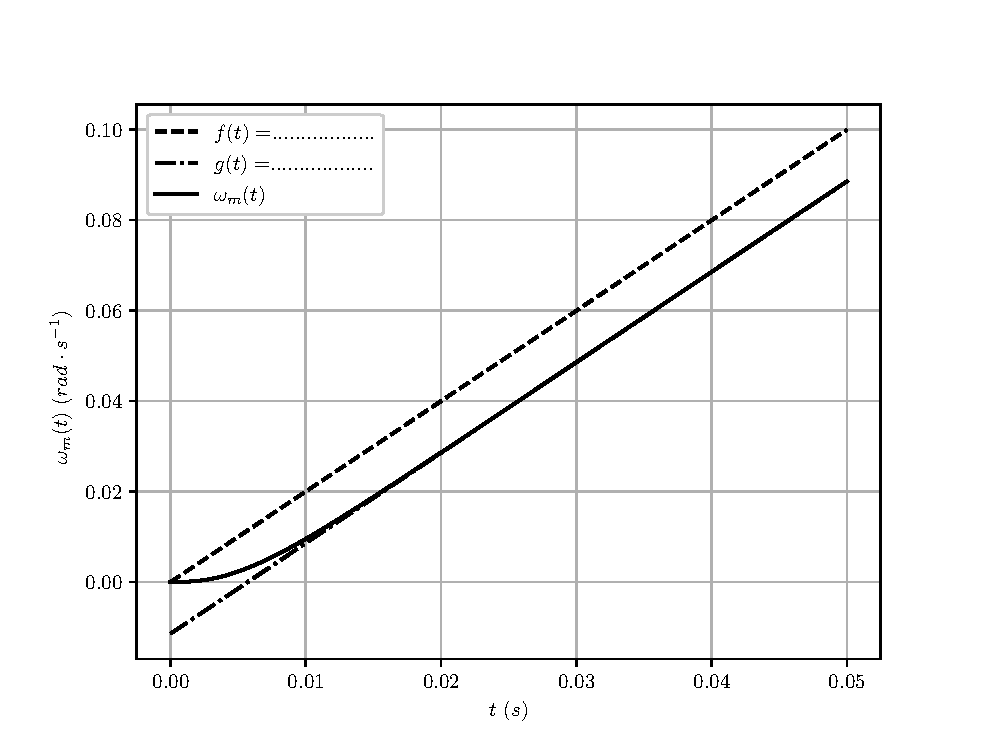
\includegraphics[width=\linewidth]{img/DR02}
\end{center}
\label{dr02}
\caption{Réponse temporelle}
\end{figure}}{\begin{figure}[ht!]
\begin{center}
 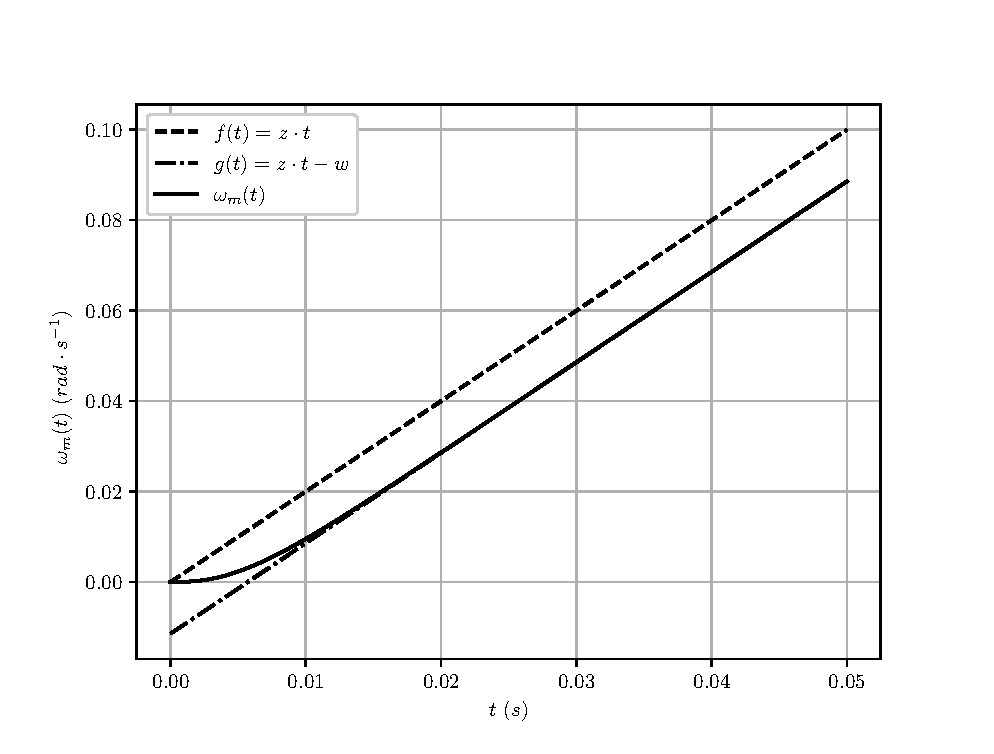
\includegraphics[width=\linewidth]{img/DR02_cor}
\end{center}
\label{dr02_cor}
\caption{Réponse temporelle}
\end{figure}}


\reponse{4}{}{$w\approx -0.01$ et $z=2$}

\newpage

\reponse{4}{}{$\delta t=0.005=5ms$.}

\reponse{0}{\begin{figure}[ht!]
\begin{center}
 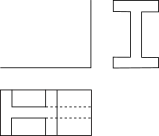
\includegraphics[width=\linewidth]{img/DR03}
\end{center}
\label{dr03}
\caption{Vue plane à compléter}
\end{figure}}{\begin{figure}[ht!]
\begin{center}
 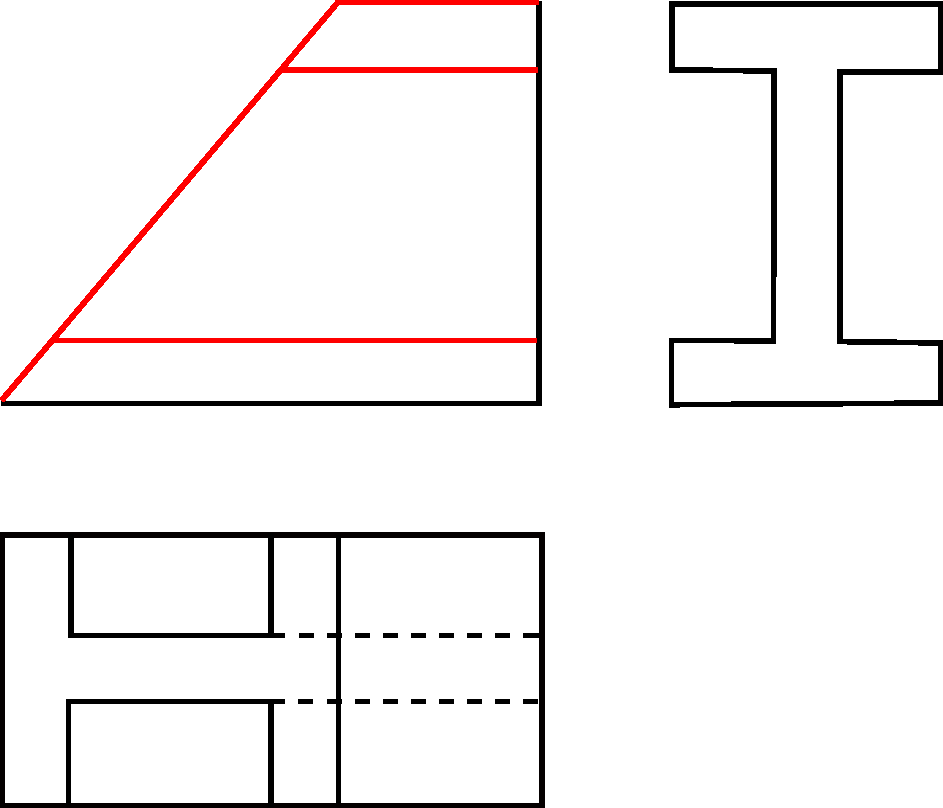
\includegraphics[width=\linewidth]{img/DR03_cor}
\end{center}
\label{dr03_cor}
\caption{Vue plane à compléter}
\end{figure}}












\end{document}
